%last updated in April 2002 by Antje Endemann

\documentclass[runningheads]{llncs}
%In order to omit page numbers and running heads
%please use the following line instead of the first command line:
%\documentclass{llncs}.
%Furthermore change the line \pagestyle{headings} to
%\pagestyle{empty}.

\input{psfig.sty}

\usepackage{graphicx}
\usepackage{epstopdf}
\usepackage{subfig}
\usepackage{array}

\begin{document}

\pagestyle{headings}
%In order to omit page numbers and running heads
%please change this line to
%\pagestyle{empty}
%and change the first command line too, see above.

\mainmatter

\title{Victim Detection from a low-altitude fixed-wing UAV: Experimental Results}

\author{Anurag Sai Vempati, Gabriel Agamennoni, Thomas Stastny, Roland Siegwart}

\titlerunning{Lecture Notes in Computer Science}

\maketitle

\begin{abstract}
This paper outlines a method to identify humans from a low-altitude fixed-wing plane relying on various Visual and Inertial sensors including an Infrared camera. The work draws inspiration from the need to detect victims trapped in a disaster situation in real-time and help the rescue units reach them. Such a work can also be easily employed for surveillance related applications. With recent advances in thermal imaging cameras, we now have the opportunity to explore more easier and reliable real-time applications. We start by pointing out various challenges that arise due to camera imperfections, viewpoint, altitude, synchronization etc. We provide a pipeline to efficiently fuse thermal and visual aerial imagery and get robust real-time detections. Confident detections are tracked across various frames and the real-time GPS locations of the victims is conveyed. Performance of our detection algorithm on various challenging datasets is provided.
\end{abstract}


\section{Introduction}
Search and Rescue is a widely researched field owing to it's numerous advantages in disaster scenarios. In cases like avalanches, a few minutes could make considerable difference in having better probability of suppressing the casualties. With increasing autonomy of the Unmanned Aerial Vehicles (UAV) and camera imaging technologies, it is now possible to scan large areas in a very short time and perform perception algorithms on-board at high rates with close to zero human intervention. Such technology also enables surveying in-accessible regions and hostile terrains making the task of dispatching rescue efforts considerably easy. In this paper we describe an algorithm that can efficiently detect trapped victims while autonomously scanning large areas using a UAV equipped with various sensors including visual and thermal cameras and an on-board computer to perform real-time computations. We will briefly outline individual components involved and provide results on a field experimental test.

Visual spectrum cameras have been used since a long time on UAVs but analyzing these images at high rates requires very robust algorithms to deal with various difficulties posed due to the size of objects of interest, motion blur, and viewpoint to name a few. Detecting humans from a UAV cruising at an altitude of 50-100 meters requires very high resolution cameras and the ability to quickly detect objects occupying few tens of pixels in area. On the other hand thermal cameras offer an advantage in such cases which makes it easier to narrow down the search space to hotter objects. But thermal cameras have their own limitations like low Signal-to-Noise Ratio (SNR), white-black/hot-cold polarity changes, and halos that appear around very hot or cold objects[IMPROVED HUMAN DETECTION AND CLASSIFICATION IN THERMAL IMAGES]. We propose a technique that best utilises the pros of either cameras using sensor fusion technique.

Various works like... leverage on hotspot techniques to quickly narrow down the potential areas to further process. [A two-stage template approach to person detection in thermal imagery] uses fast-screening technique by modelling the background as an average of previous frames. For the foreground regions template called Contour Saliency Maps (CSM) are generated that preserves the edges that are both strong and significantly different from the background. The potential regions are found by correlating this template across the image. Such averaging techniques perform poorly in case of fast moving cameras like on UAVs. Many techniques rely on some kind of classifier to detect presence of a human in each of these potential areas. [A two-stage template approach to person detection in thermal imagery], [ACtive People Recognition using thermal and gray images on a Mobile security robot], [Human Body Detection and Geolocalization for UAV Search and Rescue Missions Using Color and Thermal Imagery], [IMPROVED HUMAN DETECTION AND CLASSIFICATION IN THERMAL IMAGES] use some kind of variant of cascade of boosted classifiers introduced by [Viola and Jones] - which basically involves a series of weak classifiers each better than the previous one. [People Detection and Tracking from Aerial Thermal Views] show performance of various feature based classifiers trained on thermal data collected across wide variation in temperature, altitude and camera movement. HOG feature based classifier in conjunction with a particle filter tracker was found to perform the best.

\section{Victim Detection Pipeline}
Detecting humans from an altitude of 50-100 meters with a camera of limited resolution poses a very challenging problem. Basic blocks of our pipeline are mentioned below:-

\subsection{Datasets}

\subsection{Background Subtractor}
Fig.~\ref{fig:thermal_sample} shows a human as seen in false-color rendering of the thermal camera image at an altitude of about 70 meters. At this scale, the humans occupy less than 50 pixels ($<$0.02\%) in an image of 640 x 512 resolution. An exhaustive search for such a tiny object of interest is very time consuming. So, we propose a Background Subtractor that returns regions of interest (ROI) and narrows down the search space considerably, thus enabling real-time detection. The foreground here is defined as a part of the image whose temperature differs quite significantly from it's surroundings. Since, humans are usually hotter (in winter) or colder (in summer) than the surroundings, we propose a technique that adaptively adjusts 2 threshold values ($t_{low}, t_{high}$) based on the surrounding pixel intensities. All the pixels with intensities less than $t_{low}$ or greater than $t_{high}$ are considered as foreground pixels.

\begin{figure}
\centerline{\includegraphics[scale=0.3]{img/sample_thermal.png}}
\caption{A sample image recorded from the FLIR thermal camera at an approximate altitude of 70 meters. Two humans are pointed out.}
\label{fig:thermal_sample}
\end{figure}

We employ a very simple sliding window based approach to estimate adaptive thresholds. The image is divided into various overlapping blocks and the adaptive thresholds $t_{low}^b, t_{high}^b$ for each block $b$ is evaluated as the higher and lower quantiles of the Gaussian models fitted to the pixel intensities of the block. Now, the threshold values at each pixel location $(i, j)$ are chosen as weighted average of all the block thresholds $t_{low}^b, t_{high}^b$ if the pixel belongs to block $b$. The weights are chosen inversely proportional to the pixel's distance from the block's center. A segmentation map (segmap) is generated by thresholding the Infrared image at each pixel location.

Fig.?? shows 2 sample images collected at different altitudes, temperature and times of the day and the corresponding segmaps. A blob detection algorithm [??] is used to find blobs of desired size, thus providing ROIs to search for humans. For the UAV scenario, we further narrow down the search space by considering only the blobs whose area lies in certain range that is calculated at every time-step based on the camera specifications, mounting, UAV's IMU pose and GPS position. This approach is computationally much cheaper and is not affected by the fast moving camera. It provides much better results at real-time than our previous implementation using Vibe[??].


\begin{figure}
  \centering
  \begin{tabular}{ccc}
    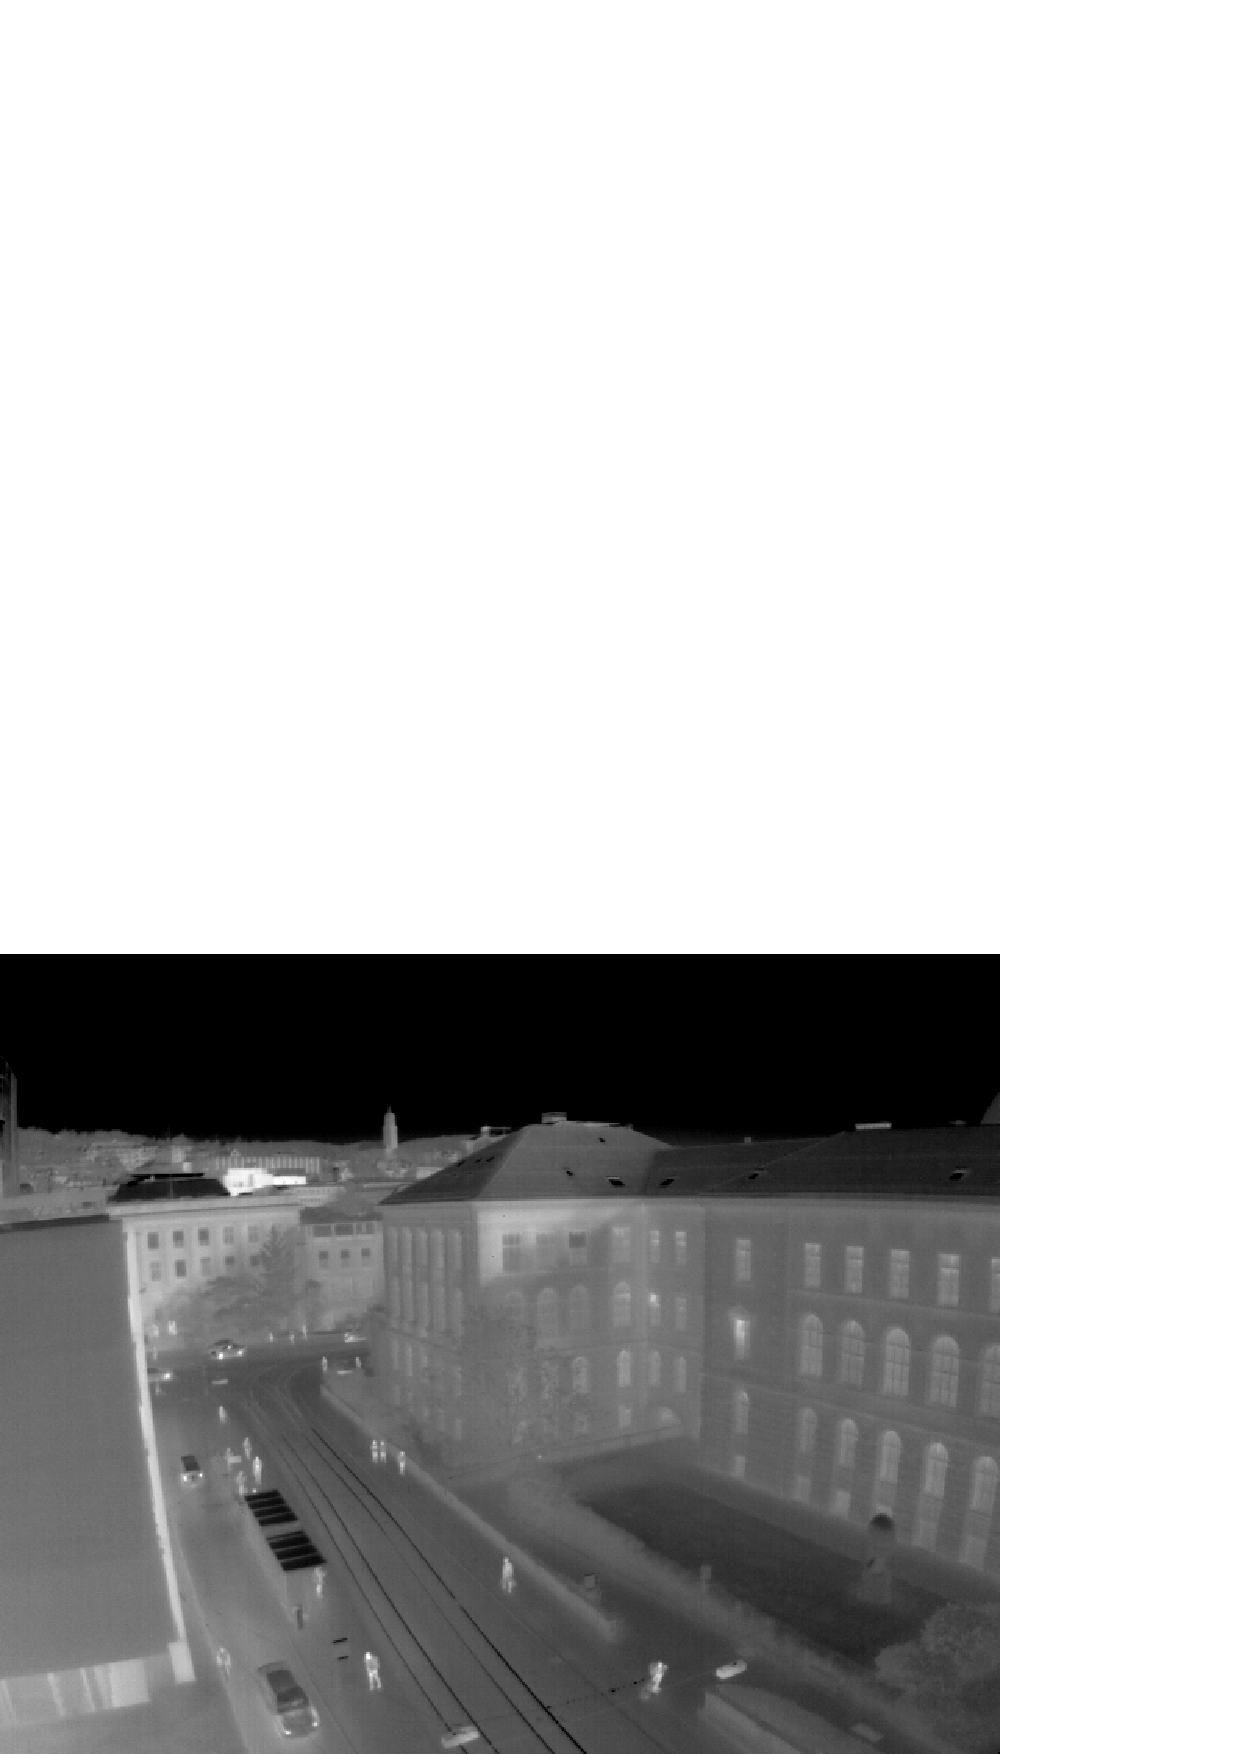
\includegraphics[width=4cm]{img/bg_sub/CLA_Infrared_Image_screenshot_03-08-2015.png} &
    \includegraphics[width=4cm]{img/bg_sub/CLA_Threshold_values(high)_screenshot_03-08-2015.png} &
    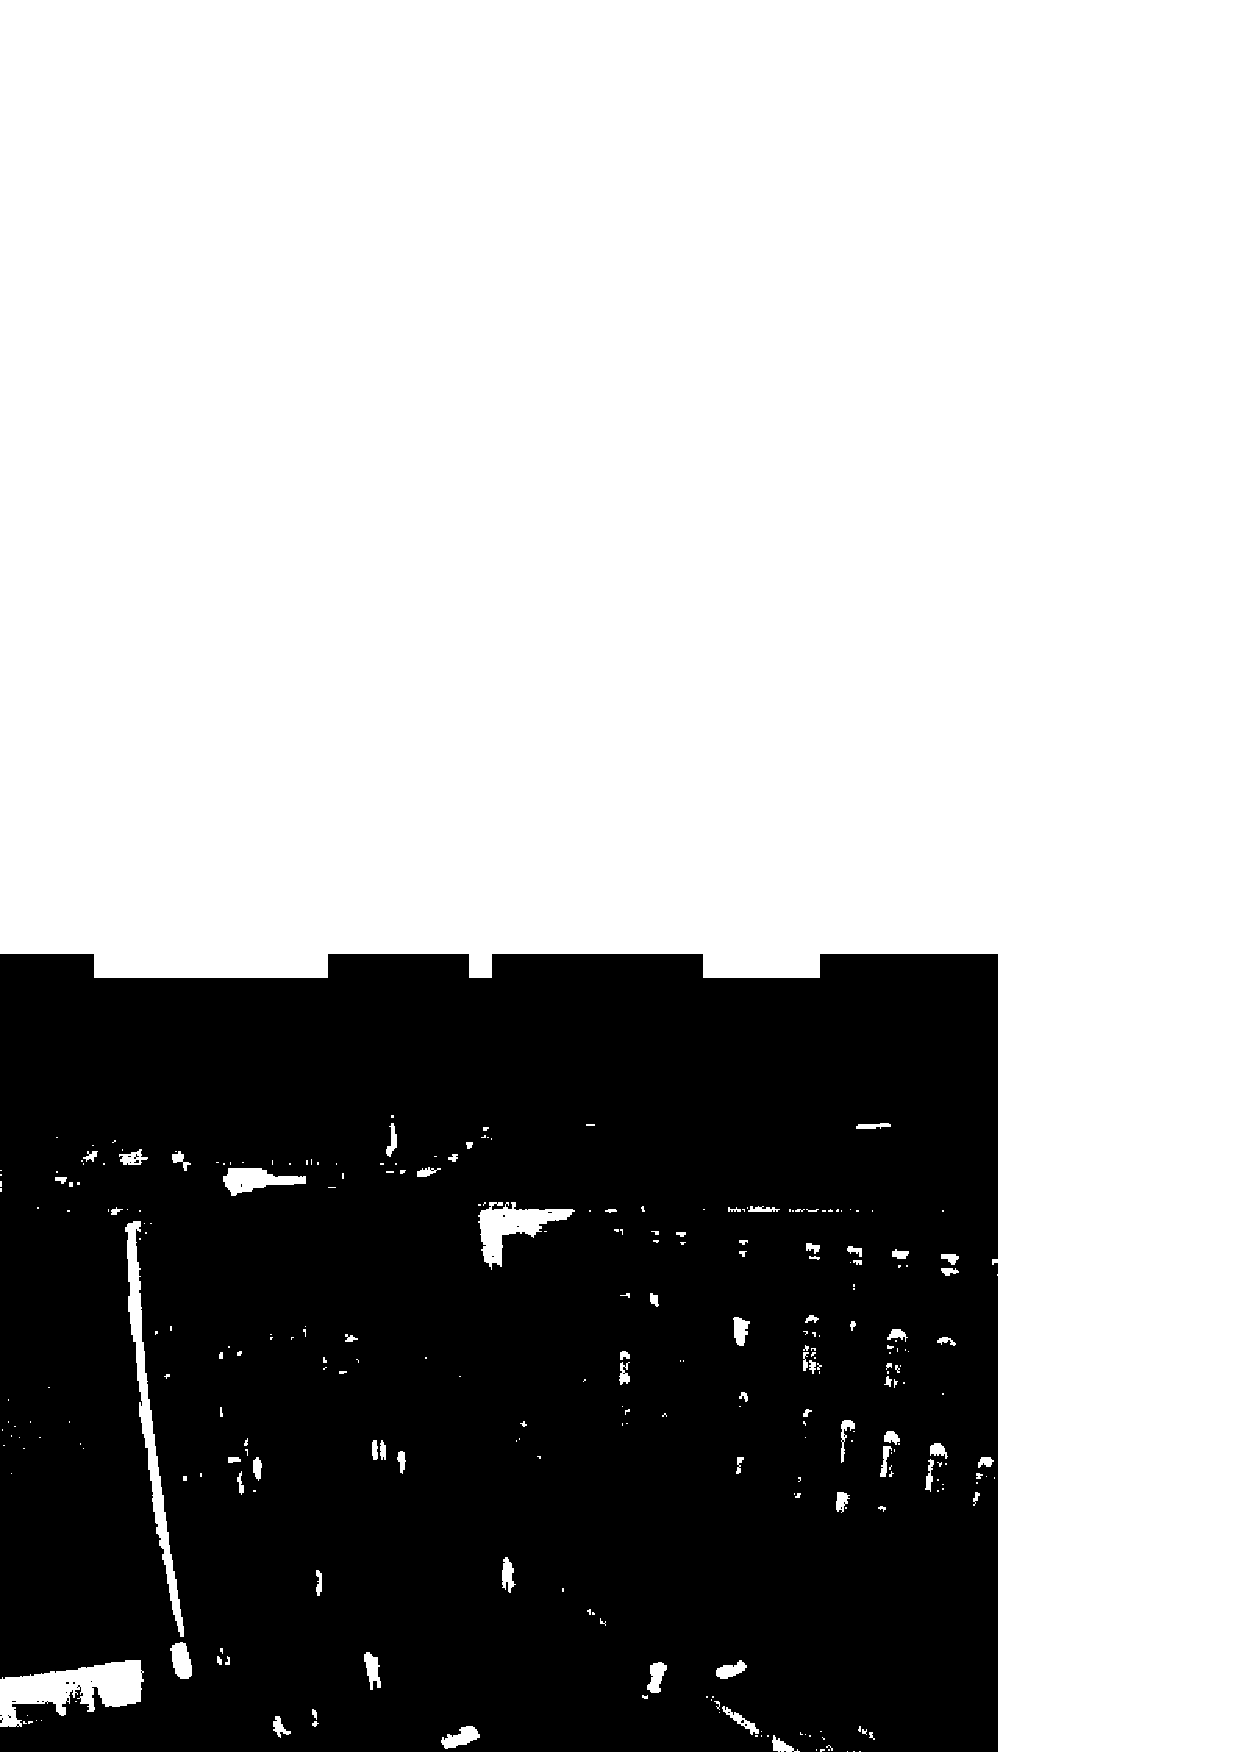
\includegraphics[width=4cm]{img/bg_sub/CLA_Segmentation_Map_screenshot_03-08-2015.png} \\
    \small (a) IR image & 
    \small (b) 8-bit threshold image &
    \small (c) Segmentation map
  \end{tabular}

  \vspace{\floatsep}

  \begin{tabular}{ccc}
    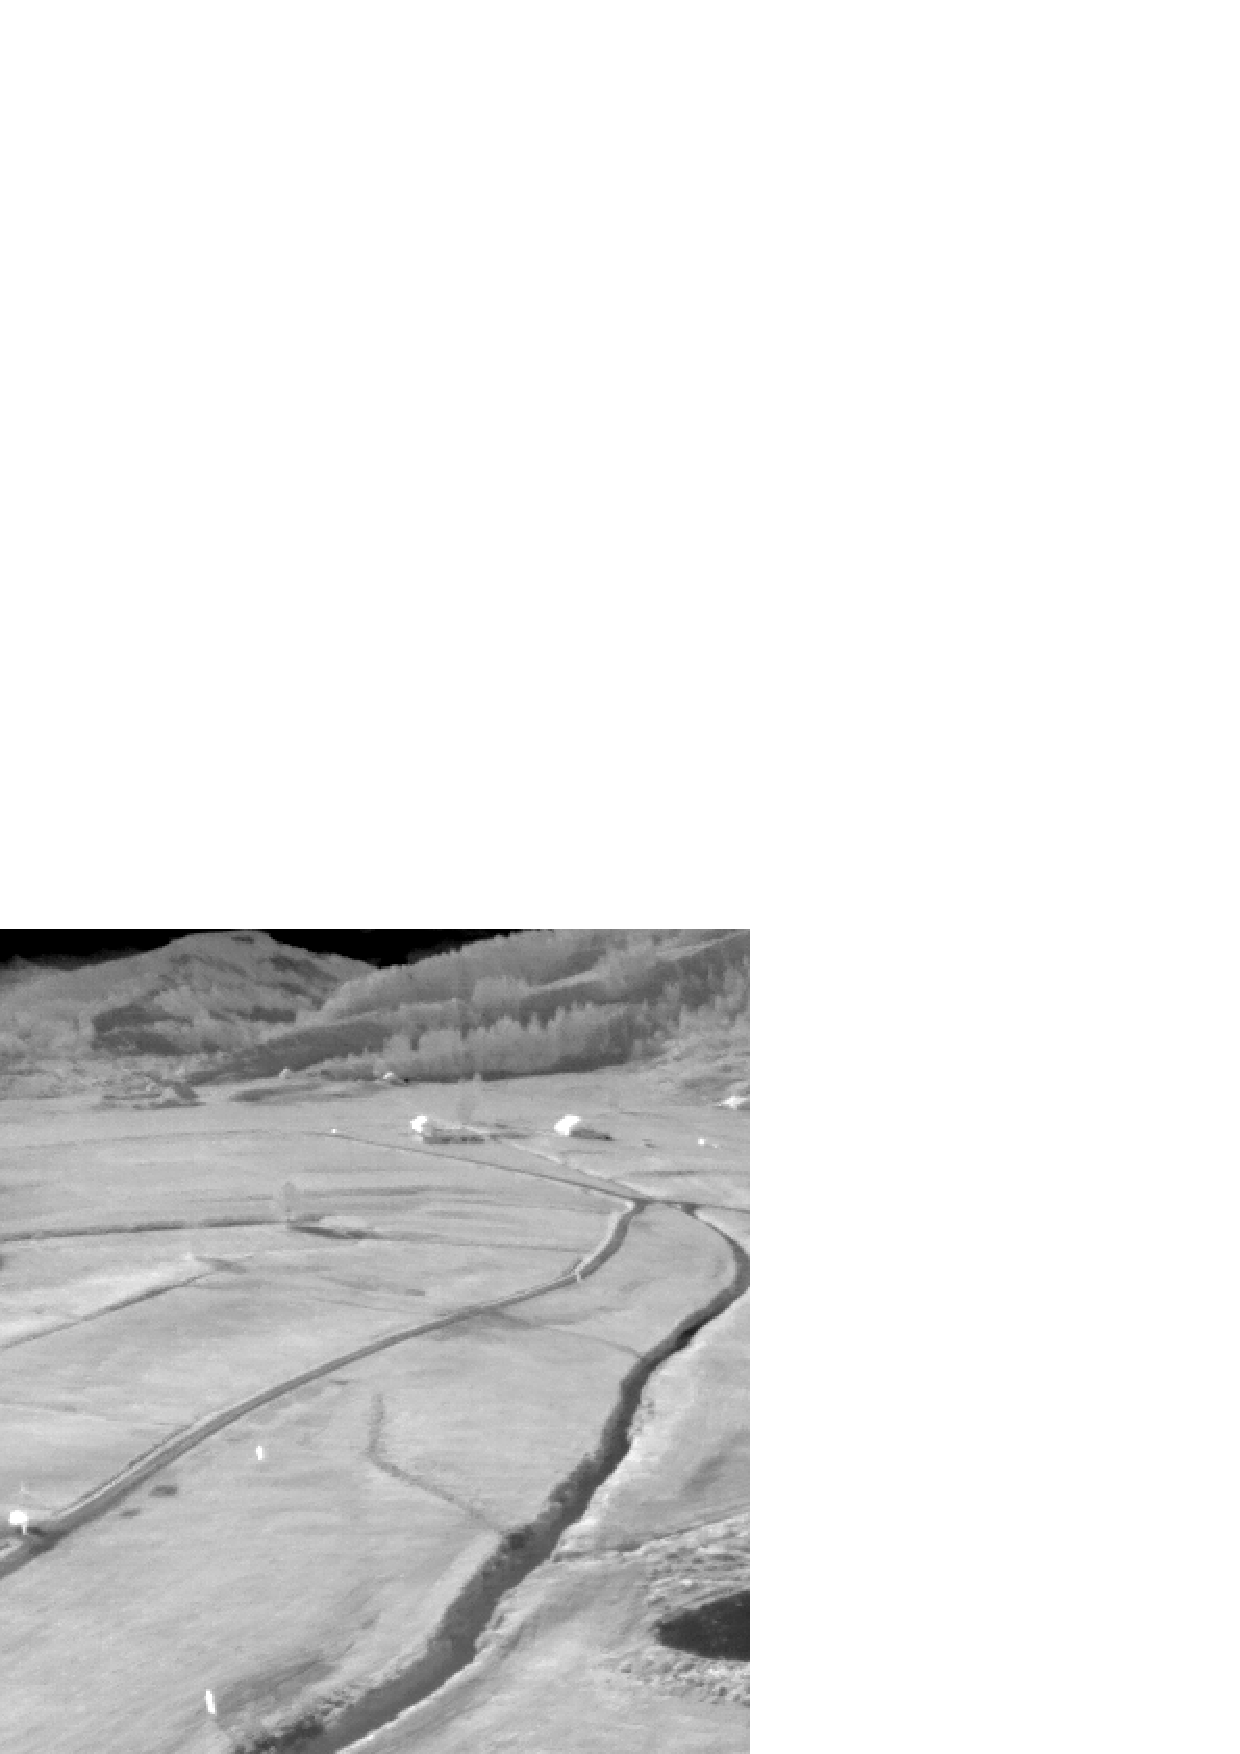
\includegraphics[height=4cm]{img/bg_sub/Roth_Infrared_Image_screenshot.png} &
    \includegraphics[height=4cm]{img/bg_sub/Roth_Threshold_values(high)_screenshot.png} &
    
\includegraphics[height=4cm]{img/bg_sub/Roth_Segmentation_Map_screenshot.png} \\
    \small (a) IR image & 
    \small (b) 8-bit threshold image &
    \small (c) Segmentation map
  \end{tabular}

  \caption{Sequence 1 is captured in the night time at an altitude of 20 meters above the ground with some crowd. Sequence 2 was captured from AS[??] on a cold winter morning at an altitude of 50 meters above the ground. (a) shows the Infrared image, (b) is the 8-bit image of pixel-wise threshold $t_{high}(i, j)$  (grid of blocks is overlaid and a sample block is marked in white on the top-left) and (c) is the resulting segmentation map depicting foreground pixels.}\label{fig:bg_sub}
\end{figure}


\subsection{Human Classifier}

The ROIs obtained from Background Subtraction are exhaustively searched for presence of a human. For this, we use a HOG feature based learning classifier (which was found to be optimal [??]) to classify the extracted patch into human or non-human category. The training data is obtained by manually annotating sequences from different datasets using vBBToolbox[??]. The distribution of training data across the datasets is shown in Table??. An SVM classifier is trained using these image patches. Type of SVM optimization problem, kernel type and other parameters are optimized using K-fold cross validation. Fig.~\ref{fig:k-fold} shows performance of few chosen configurations. C\_SVC optimization problem with Linear kernel type and RBF kernel type are found to be 2 top performing classifier configurations. 

\begin{table}
\begin{center}
\label{table:headings}
\begin{tabular}{lll}
\hline\noalign{\smallskip}
Heading level & Example & Font size and style\\
\noalign{\smallskip}
\hline
\noalign{\smallskip}
Title (centered)  & {\Large \bf Lecture Notes \dots} & 14 point, bold\\
1st-level heading & {\large \bf 1 Introduction} & 12 point, bold\\
2nd-level heading & {\bf 2.1 Printing Area} & 10 point, bold\\
3rd-level heading & {\bf Headings.} Text follows \dots & 10 point, bold
\\
4th-level heading & {\it Remark.} Text follows \dots & 10 point,
italic\\
\hline
\end{tabular}
\end{center}
\caption{Distribution of training image patches among different datasets}
\end{table}

HOG features are extracted on the image patches at multiple scales and the descriptor generated is passed on to the SVM classifier to detect the presence of humans. Fig.?? shows PR curves for the performance of classifier on CLA data.

\begin{figure}
  \centering
  \begin{tabular}{m{4cm}m{4cm}m{4cm}}
    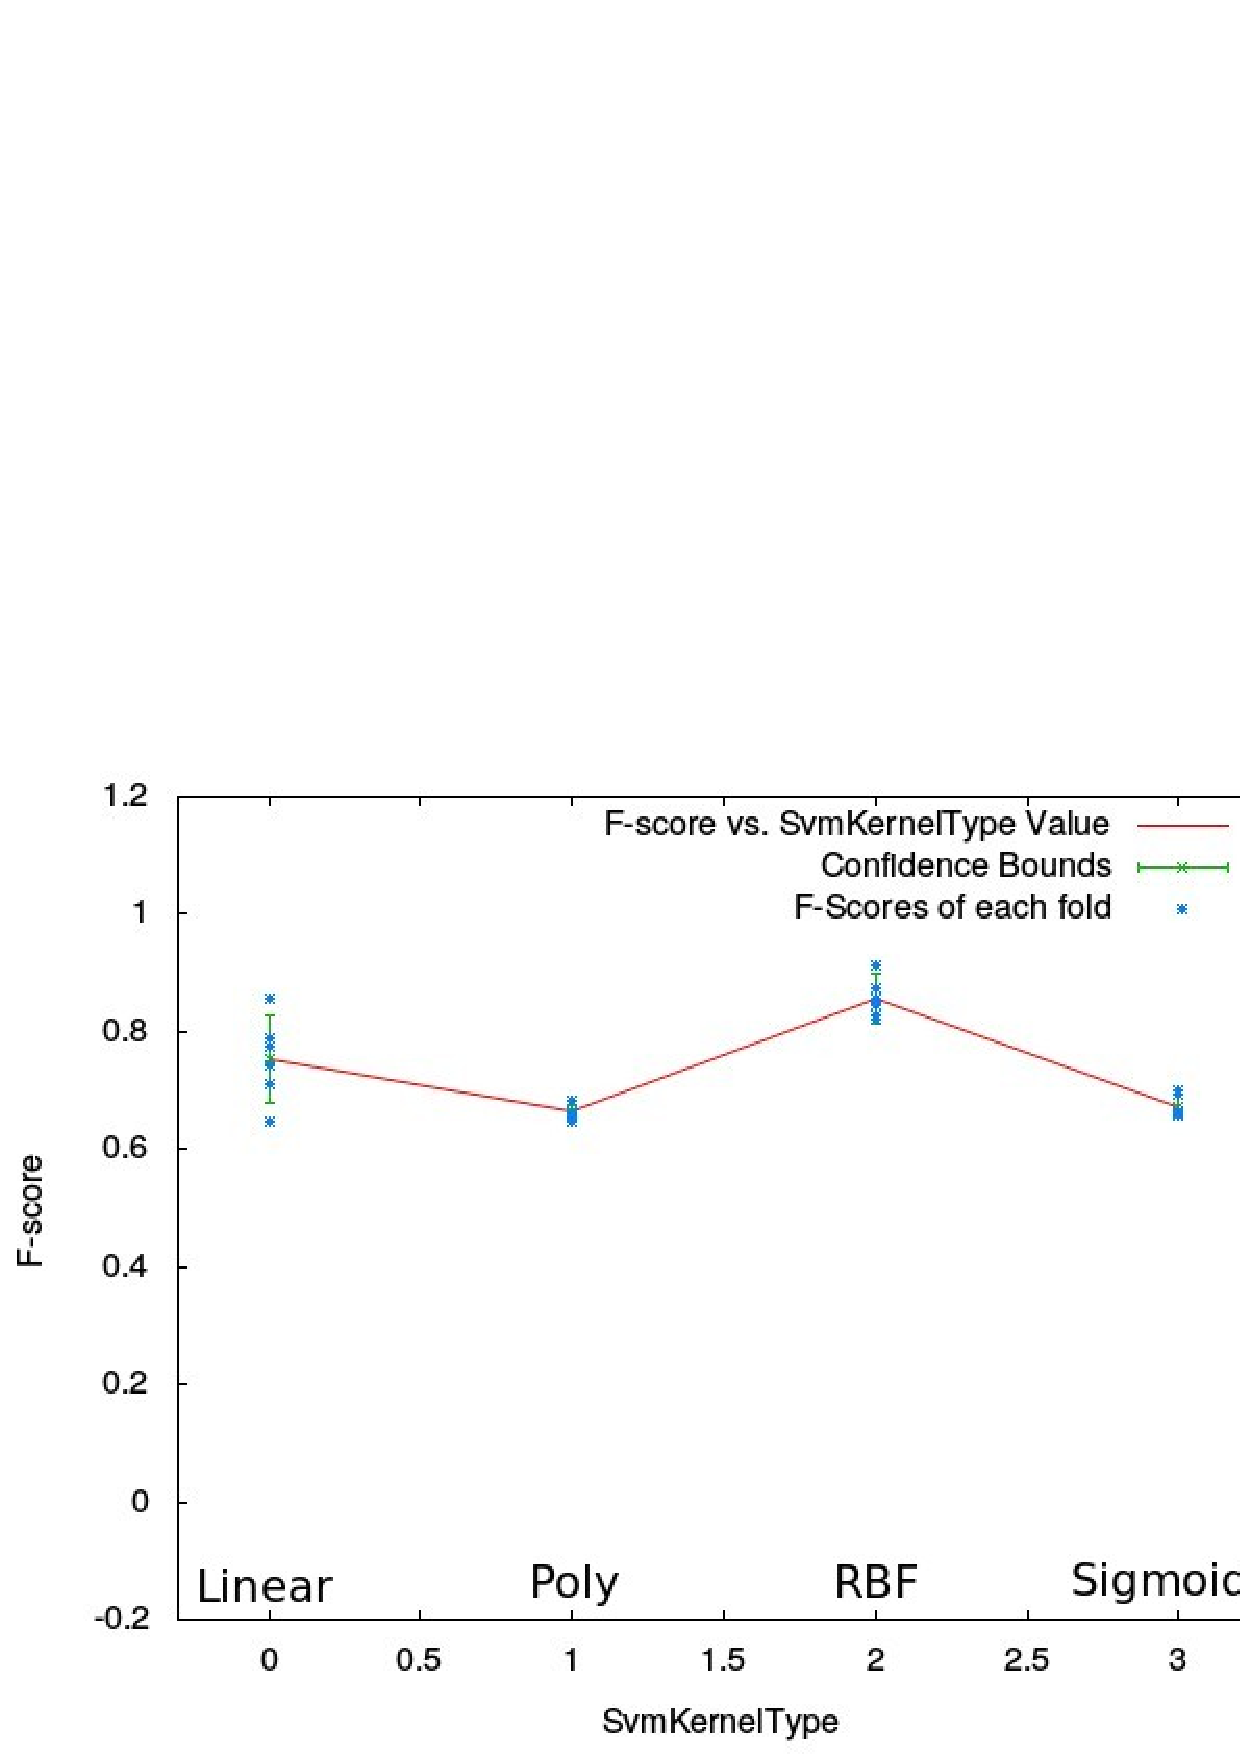
\includegraphics[width=4cm]{img/classifier/SvmKernelTypevalue_vs_score_C_SVC.jpg} &
    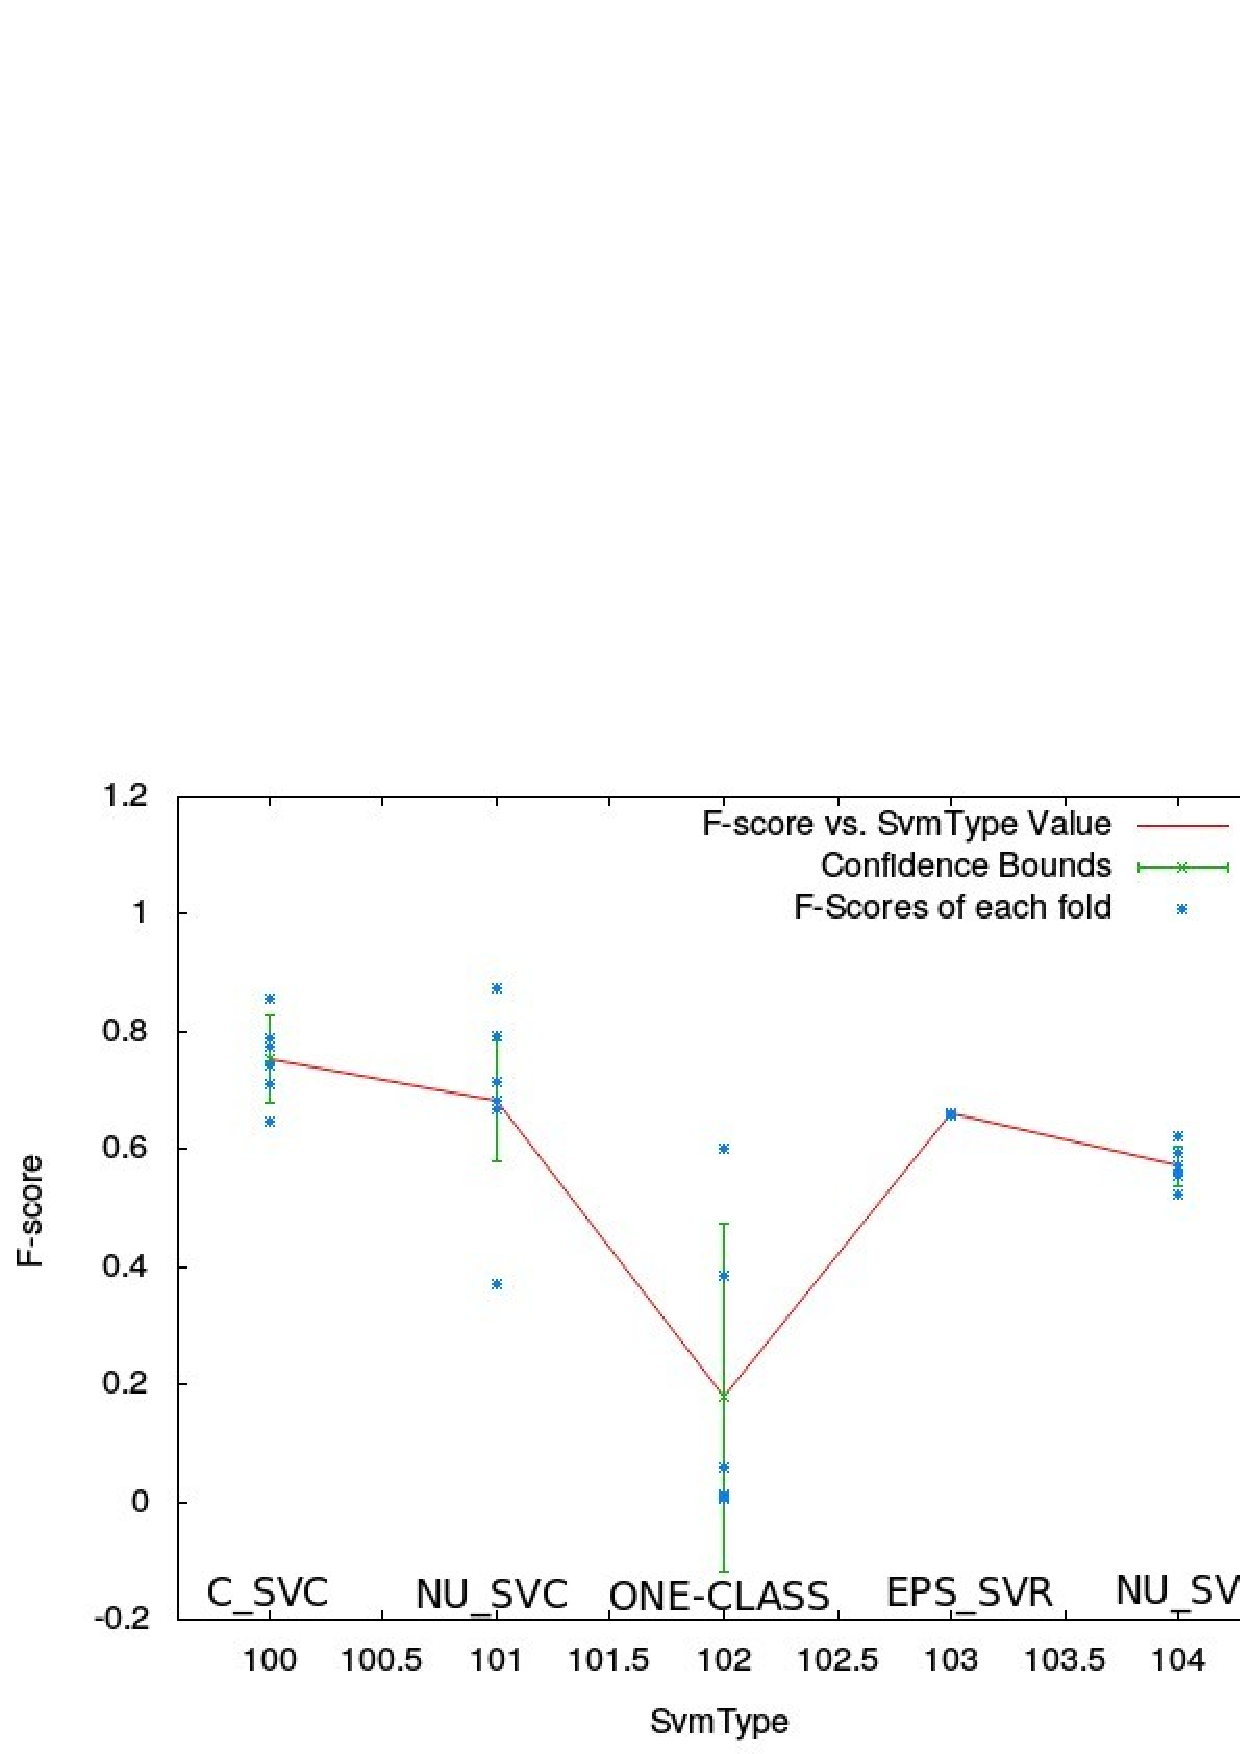
\includegraphics[width=4cm]{img/classifier/SvmTypevalue_vs_score_LINEAR.jpg} &
    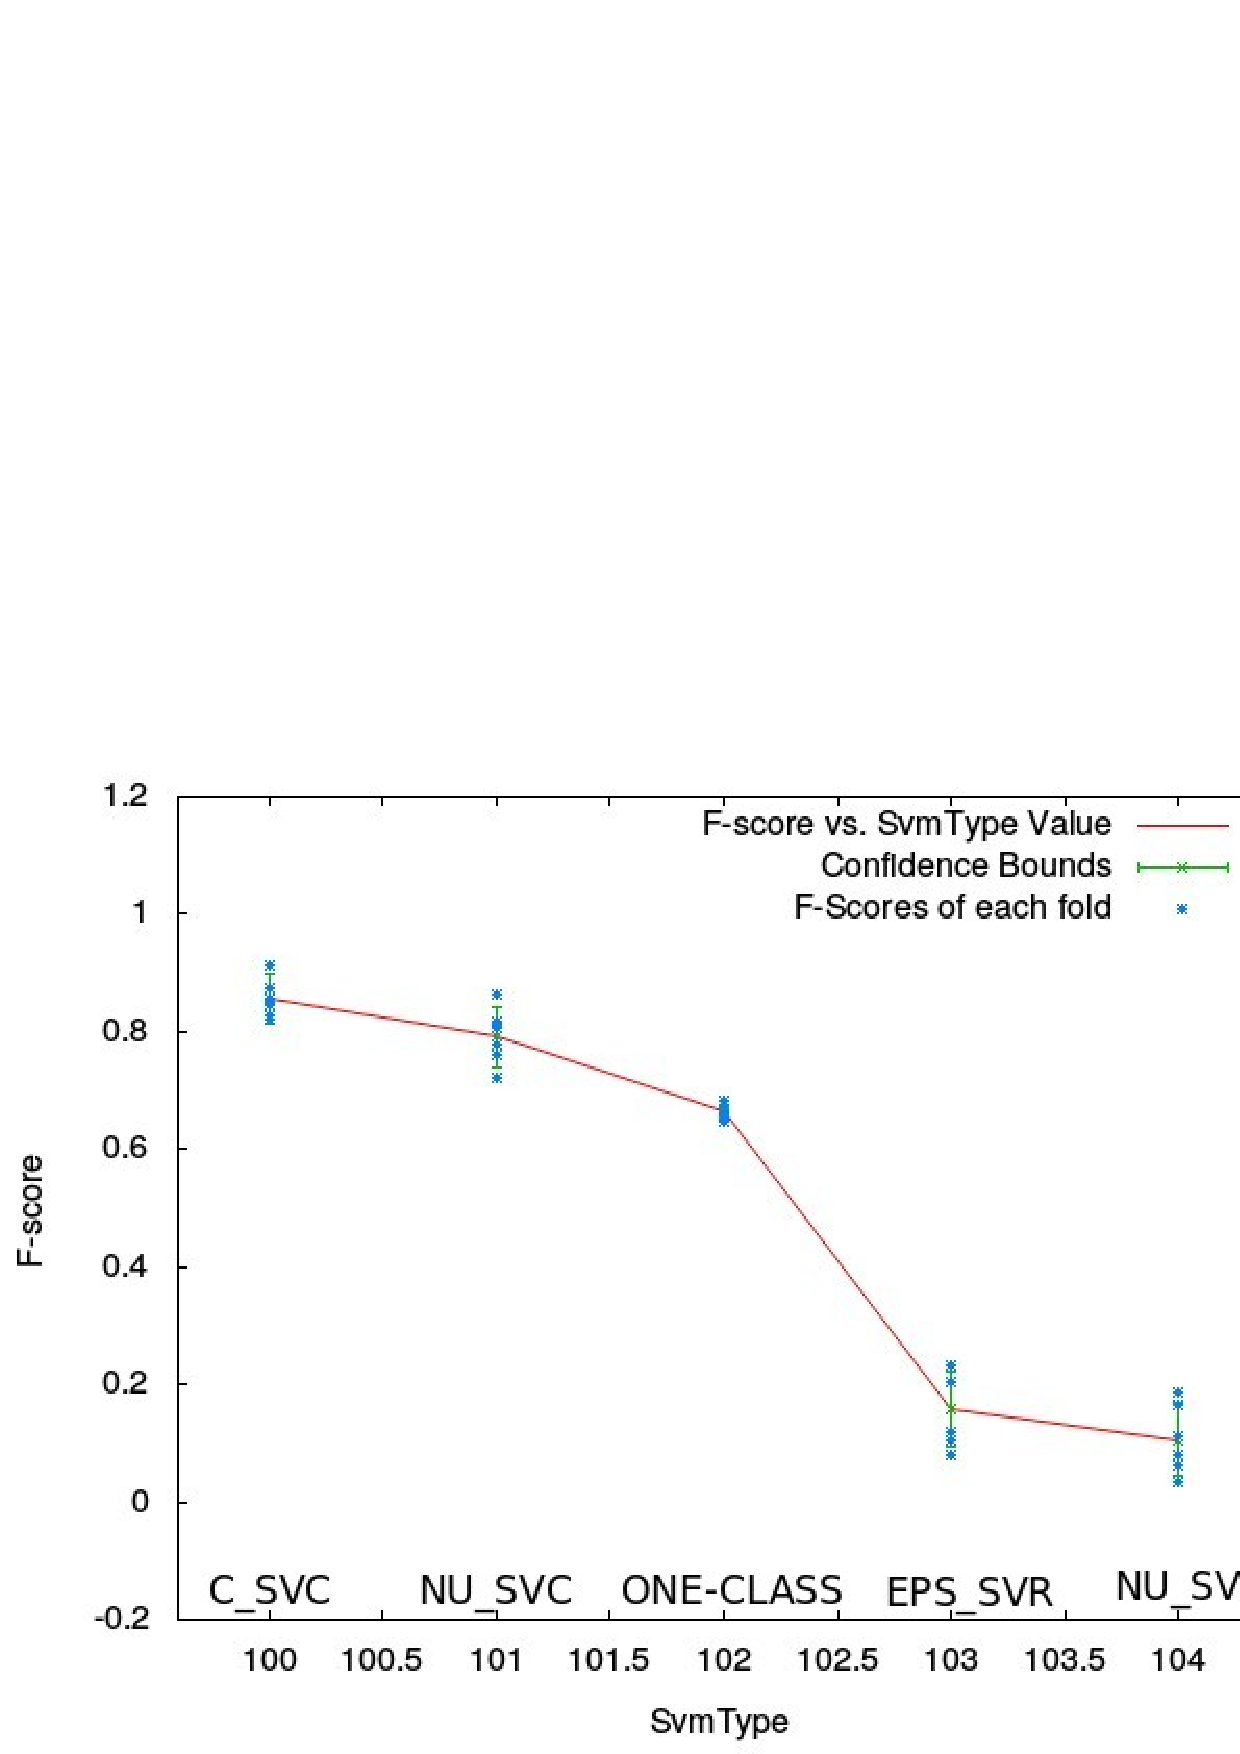
\includegraphics[width=4cm]{img/classifier/SvmTypevalue_vs_score_RBF.jpg} \\
    \tiny (a) Choosing kernel type for C\_SVC problem & 
    \tiny (b) Choosing optimization problem for linear SVM kernel &
    \tiny (c) Choosing optimization problem for RBF SVM kernel
  \end{tabular}
  
  \caption{Performance of SVM classifier with different configurations of optimization problem and kernel type. It's found to be optimal to choose (a) RBF kernel type for C\_SVC problem, (b) C\_SVC problem for Linear kernel type and (c) C\_SVC problem for RBF kernel type.}\label{fig:k-fold}
\end{figure}


<one-class SVM>


\subsection{Infrared-Grayscale Image Fusion} 

Objects in Infrared image rarely have discerning features since the temperature tends to be uniform across the objects. So, a classifier would be not so reliable in classifying such patches since it only has the shape information of the object in a very small patch. Since in all our flights using the sensorpod we collected both Infrared and Grayscale images, a fusion technique is proposed to get a one to one relationship between pixel locations of Infrared and Grayscale images. This will help us in extracting both Infrared and Grayscale image patches corresponding to the ROIs obtained from Background Subtraction which can help the classifier in producing more reliable results.

<Technique>
We use Kalibr[??] to calibrate the Infrared and Grayscale camera intrinsics and extrinsics for the sensorpod mounting. We use radial-tangential model to estimate camera distortion parameters. An april tag pattern is used to estimate Grayscale camera intrinsics. A thick matte paper with checkerboard pattern under illumination of a bright light is used to calibrate Infrared camera intrinsics. We then undistort the images and choose a new camera matrix for both the cameras with common focal parameters. An optimal camera matrix is evaluated that ensures all the original pixels are present in the final image after undistorting the images. Rotation and Transaltion matrices between the cameras is obtained using camera-camera extrinsics evaluated with Kalibr. Now the Infrared and Grayscale camera setup can be treated as a Stereo pair and standard image rectification techniques can be used to evaluate the necessary projection matrices. At this point, all the epipolar lines are parallel to image edge (horizontal if horizontal rectification was employed, vertical otherwise). For our particular setup, vertical stereo was chosen since the camera centers were aligned vertically on the sensorpod. Now that the disparities of the image are in one axis, it's fast and easy to find pixel correspondences. After a manual displacement that is set for all the columns, individual column displacements are evaluated using correspondences between fast features calculated for both the images.


Fig.~\ref{fig:fusion} shows results from the fusion technique. In Rothethurm-1 sequence IR and Grayscale cameras were both facing in the direction of flight and are $25^{\circ}$ nadir configuration with a translation of 3.5cm between the camera centers. In Sea-1 sequence, IR camera was in $25^{\circ}$ nadir configuration while Grayscale camera was in $50^{\circ}$ nadir configuration with a translation of 3.5cm between the camera centers. The results show reasonable overlap accuracy. Since, we only require a bounding box containing the same object in both Infrared and Grayscale image, this level of accuracy suffices.

\begin{figure}
  \centering
  \begin{tabular}{cccc}
    \includegraphics[width=3cm]{img/fusion/Roth/Infrared_Image_screenshot.png} &
    \includegraphics[width=3cm]{img/fusion/Roth/Grayscale_Image_screenshot.png} &
    \includegraphics[width=3cm]{img/fusion/Roth/Warped_Infrared_Image_screenshot.png} &
    \includegraphics[width=3cm]{img/fusion/Roth/Warped_Grayscale_Image_screenshot.png} \\
    \small (1.a) IR image & 
    \small (1.b) Grayscale Image &
    \small (1.c) Rectified IR &
    \small (1.d) Rectified Grayscale
  \end{tabular}

  \vspace{\floatsep}
  
  \begin{tabular}{cccc}
    \includegraphics[width=3cm]{img/fusion/Sea/3/Infrared_Image_screenshot.png} &
    \includegraphics[width=3cm]{img/fusion/Sea/3/Grayscale_Image_screenshot.png} &
    \includegraphics[width=3cm]{img/fusion/Sea/3/Warped_Infrared_Image_screenshot.png} &
    \includegraphics[width=3cm]{img/fusion/Sea/3/Warped_Grayscale_Image_screenshot.png} \\
    \small (2.a) IR image & 
    \small (2.b) Grayscale Image &
    \small (2.c) Rectified IR &
    \small (2.d) Rectified Grayscale
  \end{tabular}
  
  \vspace{\floatsep}
  
  \begin{tabular}{cc}
  	\includegraphics[width=6cm]{img/fusion/Roth/Grayscale_and_Infrared_overlaid_Image_screenshot.png} &
  	\includegraphics[width=6cm]{img/fusion/Sea/3/Grayscale_and_Infrared_overlaid_Image_screenshot.png} \\
  	\small (1.e) Fused IR and Grayscale Images &
  	\small (2.e) Fused IR and Grayscale Images
  \end{tabular}

  \caption{The top 2 rows show 2 sequences (Rothenthurm-1, Sea-1) of original images obtained from IR and Grayscale cameras and the resulting images post rectification. Last row shows fusion of 2 images to visualize the quality of overlap. Red boxes in seq-1 highlights 2 humans and a boat in seq-2. As can be seen, the correspondence between IR and Grayscale images is reasonably good.}\label{fig:fusion}
\end{figure}

Fig.?? shows improvement to the PR curves after Fusion on Roth-1 data.

\begin{figure}
  \centering
  \begin{tabular}{m{5cm}m{5cm}}
  	\includegraphics[width=6cm]{img/fusion/Roth/PR-roth-all-detections.jpg} &
  	\includegraphics[width=6cm]{img/fusion/Roth/PR-roth-top-detections.jpg} \\
  	\small (a) PR curves when all the detections are retained &
  	\small (b) PR curves when only 2 best detections per frame are retained
  \end{tabular}

  \caption{The top 2 rows show 2 sequences (Rothenthurm-1, Sea-1) of original images obtained from IR and Grayscale cameras and the resulting images post rectification. Last row shows fusion of 2 images to visualize the quality of overlap. Red boxes in seq-1 highlights 2 humans and a boat in seq-2. As can be seen, the correspondence between IR and Grayscale images is reasonably good.}\label{fig:fusion}
\end{figure}


\section{Experimental Results}

\subsection{Structural Inspection Planner}

\subsection{Estimating victim GPS}

Fig.~\ref{fig:victim_gps_small}(a) shows a schematic of all the involved sensors, the corresponding axes and the intrinsics/extrinsics involved. For estimating the GPS positions of detections, we assume the ground as a plane. Using the calibration data obtained earlier, it can be easily shown the latitude/longitude are:

Fig.~\ref{fig:victim_gps_small}(b) shows the detected victim GPS positions, actual groundtruth victim location and the path followed by the UAV. The rest of the detections include unregistered humans in the explored area and some False Positives. By enforcing a criterion - similar to [??] - that requires a particular GPS position to be detected consistently within the duration of the time that particluar spot is observed, most of the Flase Positives are eliminated and the set of true detections are registered to known groundtruths. False Positives are further eliminated by boosting the confidence of detections that are closer to the GPS location of the point where principal axis of camera hits the ground plane. Fig.~\ref{fig:victim_gps_small}(c) is a plot of GPS position estimate errors for all the 3 registered victims. The GPS estimates are converted to UTM coordinates to represent the error in meters.


\begin{figure}
  \centering
  \begin{tabular}{cc}
    \includegraphics[width=6cm]{img/victim_gps/victim_gps_on_map.jpg} &
    \includegraphics[width=6cm]{img/victim_gps/victim_gps_on_map_3.jpg} \\
    \small (a) Victim GPS for a small segment & 
    \small (b) Victim GPS
  \end{tabular}

  \vspace{\floatsep}
  
  \begin{tabular}{c}
    \includegraphics[width=11cm]{img/victim_gps/victim_utm_errors.jpg} \\
    \small (c) Victim UTM position errors
  \end{tabular}

  \caption{asdasdsadsada.}\label{fig:victim_gps}
\end{figure}














\nocite{bal:cha:gra:pae}
\bibliographystyle{splncs}
\bibliography{isvc_submission}

\section*{Appendix: Appendix Format}
The appendix should appear directly after the references, and not on a new page

\end{document}
